\documentclass{article}

\usepackage{graphicx}
\usepackage{tikz}
\usepackage{tikzsymbols}
\usetikzlibrary{calc,patterns,shapes.geometric}
\pagestyle{empty}
\usepackage[margin=0pt]{geometry}
\geometry{papersize={14in,12in}}

\def\centerarc[#1](#2)(#3:#4:#5){\draw[#1] ($(#2)+({#5*cos(#3)},{#5*sin(#3)})$) arc (#3:#4:#5);}

\begin{document}
	\begin{figure}
		\centering
		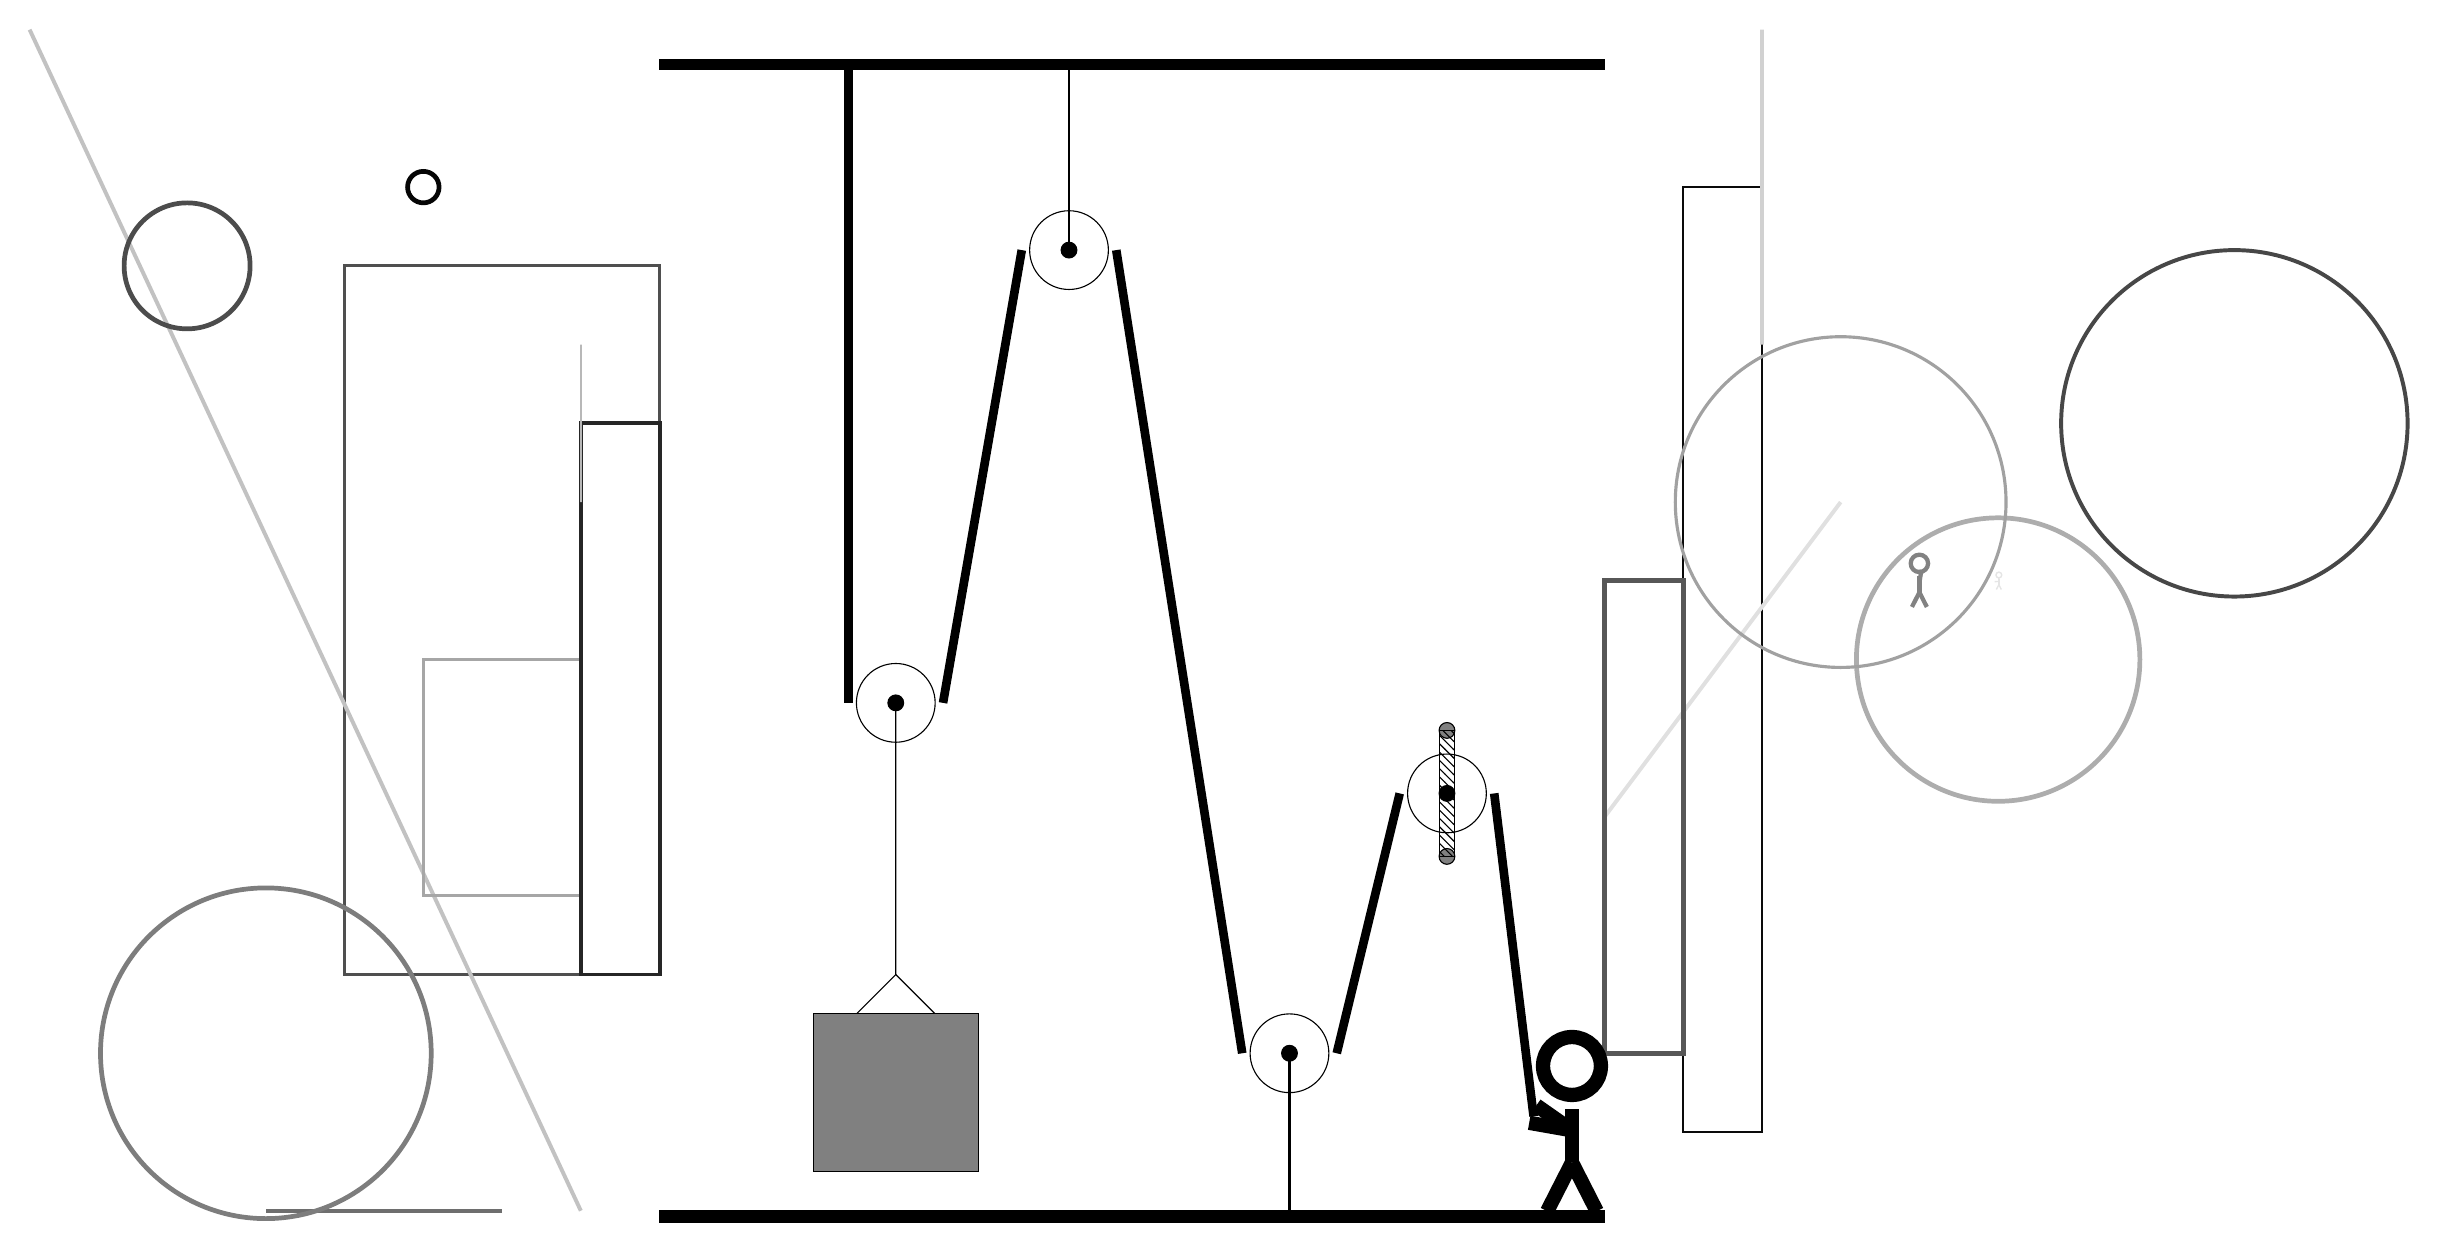
\begin{tikzpicture}
			%%%%% START %%%%%
			
			\draw[fill=black] (-2, 11.5) rectangle (10, 11.625);
			
			\draw (1, 3.45) circle (0.5);
			\draw[fill=black] (1, 3.45) circle (0.1);
			
			\draw (3.2, 9.2) circle (0.5);
			\draw[fill=black] (3.2, 9.2) circle (0.1);
			\draw[thick] (3.2, 9.2) -- (3.2, 11.5);
			
			\draw (6, -1) circle (0.5);
			\draw[fill=black] (6, -1) circle (0.1);
			\draw[thick] (6, -1) -- (6, -3);
			
			\draw[fill=white](8, 2.3) circle (0.5);
			\draw[fill=black] (8, 2.3) circle (0.1);
			\draw[fill=black!50] (8, 3.1) circle (0.1);
			\draw[fill=black!50] (8, 1.5) circle (0.1);
			\draw[pattern=north west lines, pattern color=black] (7.9, 3.1) rectangle (8.1, 1.5);
			
			\draw (1, 3.45) -- (1, 0.0) -- (0.5, -0.5);
			\draw (1, 0.0) -- (1.5, -0.5);
			\draw[fill=black!50] (-0.05, -0.5) rectangle (2.05, -2.5);
			
			\node[line width=0.7mm, color=black!10] at (15, 5) {\Strichmaxerl[1][2][89]};
			
			\draw[line width=0.5mm, color=black!57](-4, -3) -- (-7, -3);
			\draw[line width=0.4mm, color=black!69] (-2, 0) rectangle (-6, 9);
			\draw [line width=0.6mm, color=black!51](-7, -1) circle (2.1);
			\draw[line width=0.5mm, color=black!24](-3, -3) -- (-10, 12);
			\node[line width=0.5mm, color=black!49] at (14, 5) {\Strichmaxerl[3][90][81]};
			\draw [line width=0.5mm, color=black!72](18, 7) circle (2.2);
			\draw[line width=0.2mm, color=black!96] (11, -2) rectangle (12, 10);
			\draw[line width=0.4mm, color=black!35] (-3, 1) rectangle (-5, 4);
			\draw[line width=0.5mm, color=black!85] (-3, 7) rectangle (-2, 0);
			
			\draw[line width=0.5mm, color=black!12](13, 6) -- (10, 2);
			\draw [line width=0.6mm, color=black!98](-5, 10) circle (0.2);
			\draw[line width=0.6mm, color=black!66] (11, 5) rectangle (10, -1);
			
			\draw [line width=0.6mm, color=black!32](15, 4) circle (1.8);
			\draw[line width=0.2mm, color=black!28] (-3, 6) rectangle (-3, 8);
			\draw [line width=0.4mm, color=black!37](13, 6) circle (2.1);
			
			\draw[line width=0.3mm, color=black!86] (-3, 10) rectangle (-3, 10);
			
			\draw [line width=0.6mm, color=black!70](-8, 9) circle (0.8);
			\draw[line width=0.5mm, color=black!18] (12, 12) rectangle (12, 8);
			
			\draw[line width=1.1mm] (0.4, 11.5) -- (0.4, 3.45);
			\centerarc[line width=1.1mm](1, 3.45)(180:360:0.6);
			\draw[line width=1.1mm](1.6, 3.45) -- (2.6, 9.2);
			\centerarc[line width=1.1mm](3.2, 9.2)(0:180:0.6);
			\draw[line width=1.1mm](3.8, 9.2) -- (5.4, -1);
			\centerarc[line width=1.1mm](6, -1)(180:360:0.6);
			\draw[line width=1.1mm](6.6, -1) -- (7.4, 2.3);
			\centerarc[line width=1.1mm](8, 2.3)(0:180:0.6);
			\draw[line width=1.1mm](8.6, 2.3) -- (9.1, -1.8);
			
			\node at (9.5, -1.9) {\Strichmaxerl[10][-35][170]};
			
			\draw[fill=black] (-2, -3) rectangle (10, -3.15);
			
			%%%%% END %%%%%
		\end{tikzpicture}
	\end{figure}	
\end{document}